
\section{HRL}

\begin{frame}{Decomposition}
\begin{itemize}
    \item known as the MAXQ decomposition
    \begin{itemize}
        \item has both a procedural semantics -  as a subroutine hierarchy
        \item ans a declarative semantics - as a representation of the value function of a hierarchy
    \end{itemize}
    \item It is based on the assumption that the programmer can identify useful subgoals and define subtasks that achieve these subgoals
    \item By defining such subgoals, the programmer \alert{constrains the set of policies} that need to be considered during reinforcement learning
    \item {\color{red}The decomposition also creates opportunities to exploit state abstractions, so that individual MDPs within the hierarchy can ignore large parts of the state space.}
    \end{itemize}
\end{frame}

\begin{frame}{Online model-free learning algorithm, MAXQ-Q}
    \begin{itemize}
        \item learns a representation of the value function
        \begin{itemize}
            \item \alert{it makes it possible to compute and execute an improved, non-hierarchical policy via a procedure similar to the policy improvement step of policy iteration}
        \end{itemize}
        \item 
    \end{itemize}
\end{frame}

\begin{frame}{Framework de Aprendizado por Reforço (MDP)}
    \begin{figure}
        \centering
        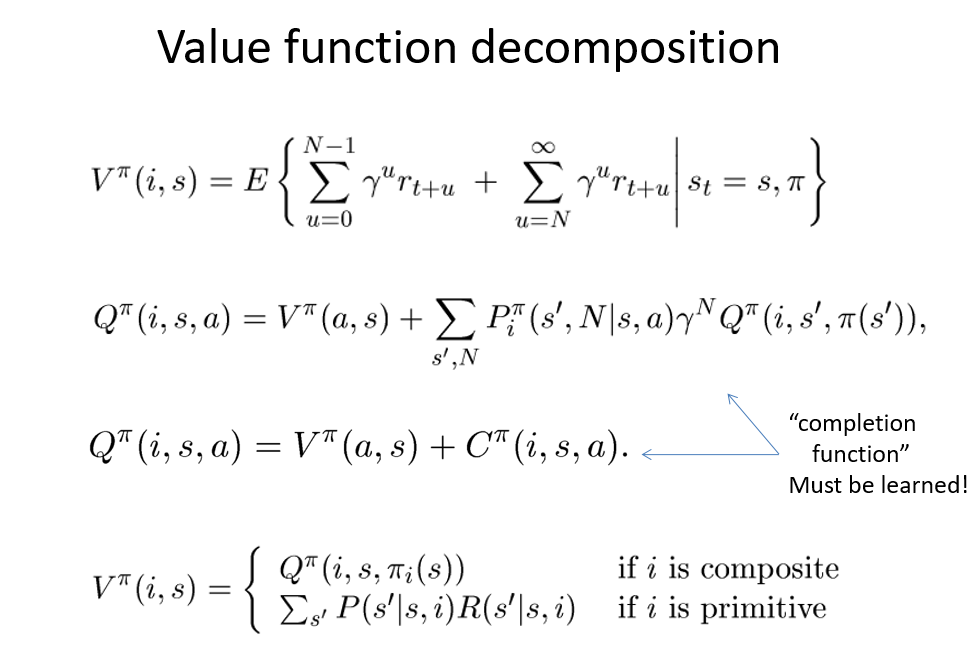
\includegraphics[width=0.7\textwidth]{img/valueFunctionDecomposition.png}
        \caption{Caption}
        \label{fig:my_label}
    \end{figure}
\end{frame}

\begin{frame}{Framework de Aprendizado por Reforço (MDP)}
    \begin{figure}
        \centering
        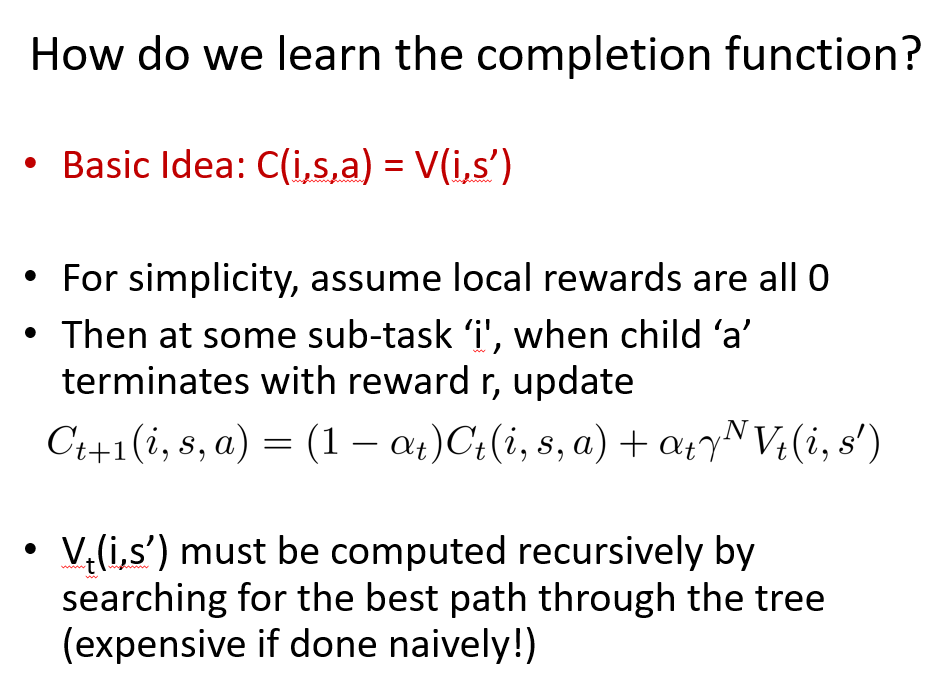
\includegraphics[width=0.7\textwidth]{img/completion_function.png}
        \caption{Caption}
        \label{fig:my_label}
    \end{figure}
\end{frame}

\begin{frame}{SMDP}
    \begin{itemize}
        \item the trajectory of system states between decision epochs in general has no effect on the state transition matrix, and as such gives the decision maker no information \cite{Mahadevan97selfImprovingFactory}
        \item the SMDP represents snapshots of the system at decision points, whereas the so-called natural process describes the evolution of states over all times \cite{Mahadevan97selfImprovingFactory}
    \end{itemize}
\end{frame}

\begin{frame}{Options - Generalização de ações para incluir cursos de ações \nocite{SatinderSingh}}
    \begin{block}{Opção}
        Uma opção é a tupla $o = <I, \pi, \beta>$
        \begin{itemize}
            \item $I \subseteq S$ é o conj de estados em que $o$ pode ser iniciado;
            \item $\pi:S \times A \rightarrow [0,1]$ é a política seguida durante $o$
            \item $\beta:S \rightarrow [0,1]$ é a probabilidade de terminar em cada estado
        \end{itemize}
    \end{block}
    \begin{block}{}
    A execução da opção é assumida ser \alert{call-and-return}
    Opções pode realizar variados números de passos.
    \end{block}
\end{frame}

\subsection{Q Learning}
\begin{frame}{Q Learning}
    \begin{itemize}
        \item MDP:
        \begin{enumerate}
            \item existe uma única função valor ótima $Q^*(s,a)$; e
            \item existe pelo menos uma política ótima $\pi^*$
            $$\pi^*(s,a) > 0, \text{se} a \in arg \max_{a' \in \mathcal{A}}Q^*(s,a')$$
        \end{enumerate}
        \item Q-learning (Watkins, 1989) (Stole et al, 2012) \nocite{stolle2002learning}
        $$Q(s_t,a_t) \leftarrow Q(s_t, a_t) + \alpha(r_{t+1} + \gamma \max_{a' \in \mathcal{A}}Q(s_{t+1},a_{t+1}) - Q(s_t, a_t)) $$
    \end{itemize}
    \vspace{20pt}%em, ex, in, pt, pc, cm, mm, dd, cc, nd, nc, bp, sp
    \centering
    \alert{O Q-learning converge no limite, com probabilidade 1, à função valor ótima $Q^*$, sob aproximação estocástica.}
\end{frame}

\subsection{Q Learning com Opções}

\begin{frame}{Q Learning com Opções}
    \begin{itemize}
        \item Uma opção é especificada por um conjunto de estados no qual a opção pode \alert{ser iniciada, usar uma política interna e ter uma condição terminal}. \nocite{stolle2002learning}
        \item Opções são generalizações de ações primitivas para incluir \alert{cursos de ação temporariamente estendidos}. \nocite{precup2000temporal, Sutton1999a}
            
        \item Uma \alert{opção $(I, \pi, \beta)$} é avaliada no estado $s_t$ se e somente se $s_t \in I $:
        \begin{itemize}
            \item política $\pi:S \times A \rightarrow [0,1]$;
            \item condição terminal $\beta : S^+ \rightarrow [0,1]$
            \item um conjunto de inicialização $I \subseteq S$
        \end{itemize}
        \item Se a opção é tomada, então ações são selecionadas de acordo com $\pi$ até a opção terminar estocasticamente conforme $\beta$
    \end{itemize}
\end{frame}

\begin{frame}{Q Learning com Opções}
    \framesubtitle{Learning with options - SMDP value learning}
    \begin{itemize}
        \item Execution of option:
        \begin{itemize}
            \item o is started in state s
            \item s' at termination of o 
            \item So, an approximate option-value function Q(s,o) is updated
        \end{itemize}
    \end{itemize}
    $$Q(s,o) \leftarrow Q(s,o) + \alpha \left [ r + \gamma^k \max_{o' \in \mathcap{O_{s'}} } Q(s',o') - Q(s,o)\right ]$$
    \begin{itemize}
        \begin{itemize}
            \item k: é o número de passos temporais entre s e s'
            \item r: é a recompensa descontada acumulada
            \item $\alpha$: pode depender arbitrariamente do estado, opção e passos temporais
        \end{itemize}
    \end{itemize}
\end{frame}

\begin{frame}{Q Learning com Opções}
    \framesubtitle{Learning with options - SMDP value learning}
    \begin{itemize}
        \item opções selecionadas pelo método $\epsilon-greedy | \epsilon = 0.1$
        \begin{itemize}
            \item opções selecionadas de forma aleatória a partir daquelas opções com valores máximo ($Q(s_t, o_t) = max_{o \in O_{s_t}} Q(s_t, o)$)
            \item probabilidade $\epsilon$ seleção aleatória para todas as opções disponíveis
        \end{itemize}
    \end{itemize}
    \begin{figure}
        \centering
        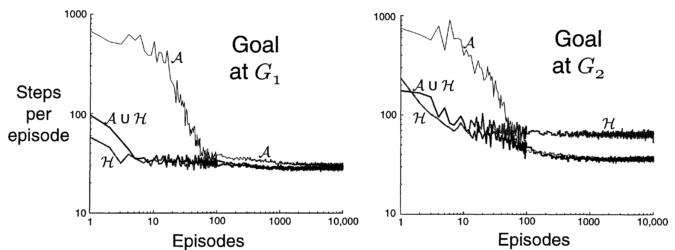
\includegraphics[width=0.7\textwidth]{img/learningOptions.png}
        \label{figLearningOptions}
    \end{figure}
\end{frame}

\begin{frame}{Q Learning com Opções}
    \framesubtitle{Interrupting options}
    \begin{itemize}
        \item interrupting options before they would terminate naturally according to their termination conditions \nocite{Sutton1999a}
        %Suppose we have determined the option-value function Qµ(s,o) for some policy µ and for all state-option pairs s, o that could be encountered while following µ. This function tells us how well we do while following µ, committing irrevocably to each option, but it can also be used to re-evaluate our commitment on each step.
        \item Se $o$ é Markov em $s_t$, então podemos comparar o valor de continuar com $o$, onde $Q_\mu(s_t, o)$, ao valor de interromper $o$ e selecionar uma nova opção de acordo com $\mu$, onde $V^\mu(s)=\sum{_q}{\mu(s,q)Q^{\mu}(s,q)}$
        \item  effect—improved performance by interrupting a temporally extended substep based on a value function found by planning at a higher level—may
        \item Termination condition $\beta$ of o' is the same as that of o except that $β'(s) = 1$ if $Q^{\mu}(s,o) < V^{\mu}(s)$
        \begin{itemize}
            \item $\mu'$ politica interrompida de $\mu$
        \end{itemize}
    \end{itemize}
\end{frame}

\begin{frame}{Q Learning com Opções}
    \framesubtitle{Interrupting options}
    \begin{figure}
        \centering
        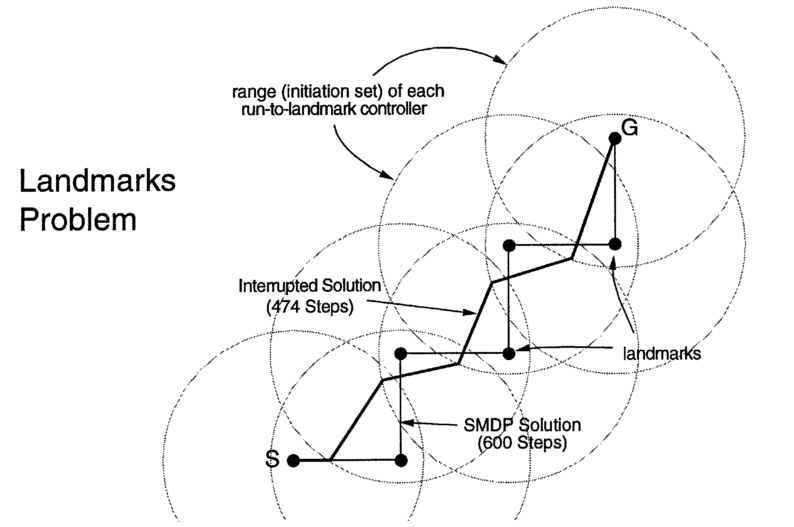
\includegraphics[width=0.7\textwidth]{img/landmarkProblem.png}
        \label{figLandmarkProblem}
    \end{figure}
    \begin{itemize}
        \item task is to navigate from a start location to a goal location within a continuous two-dimensional state space
    \end{itemize}
\end{frame}

\begin{frame}{Q Learning com Opções}
    \framesubtitle{Interrupting options}
    \begin{itemize}
        \item actions aremovements of 0.01 in any direction from the current state
        \item introduce seven landmark locations in the space
        \item Each controller is only applicable within a limited range of states, in this case within a certain distance of the corresponding landmark
        \item Each controller then defines an option: the circular region around the controller’s landmark is the option’s initiation set, the controller itself is the policy, and arrival at the target landmark is the termination condition
        \item We denote the set of seven landmark options by O. Any action within 0.01 of the goal location transitions to the terminal state, the discount rate γ is 1, and the reward is 1 on all transitions, which makes this a minimum-time task
    \end{itemize}
\end{frame}

\begin{frame}{Q Learning com Opções}
    \framesubtitle{Interrupting options}
    \begin{figure}
        \centering
        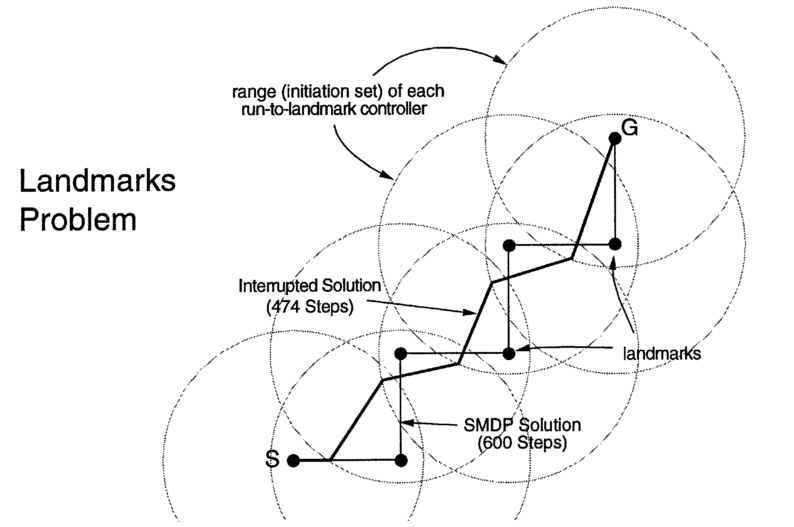
\includegraphics[width=0.5\textwidth]{img/landmarkProblem.png}
        \label{figLandmarkProblem}
    \end{figure}
    \begin{itemize}
        \item The trajectory shown by the thick line in Fig. 7 cuts the corners and is shorter. This is the interrupted policy with respect to the SMDP-optimal policy
        \item The interrupted policy takes 474 steps from start to goal which, while not as good as the optimal policy in primitive actions (425 steps), is much better, for nominal additional cost, than the SMDP- optimal policy, which takes 600 steps
    \end{itemize}
\end{frame}


\begin{frame}{Q Learning com Opções}
    \framesubtitle{Interrupting options}
    \begin{figure}
        \centering
        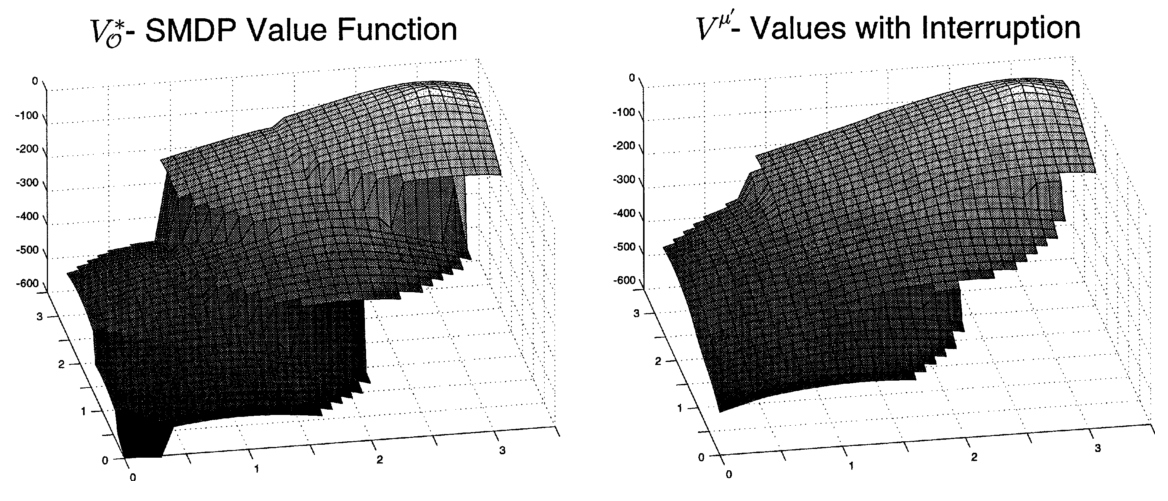
\includegraphics[width=0.7\textwidth]{img/valueFunctionInterruptingOption.png}
        \label{figLandmarkProblem}
    \end{figure}
    \begin{itemize}
        \item The thin line shows the SMDP solution, the optimal behavior that uses only these controllers without interrupting them, and the thick line shows the corresponding solution with interruption, which cuts the corners.
    \end{itemize}
\end{frame}

\subsection{Q Learning com Opções a serem Aprendidas}

\begin{frame}{Learning Options}
    \begin{itemize}
        \item options provides a natural way of incorporating temporally extended actions into reinforcement learning systems
        \item but leaves open the issue of how good options might be identi-fied.\nocite{stolle2002learning}
    \end{itemize}
\end{frame}

\begin{frame}{}
    \textbf{function} \mathcal{LearningOptions($\alpha, \gamma, \epsilon$)}\\
    %\hspace{10} $\gamma \leftarrow 0.9$, $\alpha \leftarrow 0.1$, $\epsilon \leftarrow 0.1$\\
    \hspace{10} $r \leftarrow \{g \in S\}$ \\
    \hspace{10} \textbf{repeat} until 30 runs\\
    \hspace{20} \textbf{for} each four location\\
    \hspace{30} \textbf{repeat} for 150 episodes\\
    \hspace{40} \textbackslash{}\textbackslash{} \textit{use fixed goals location}\\
    \hspace{50} s = rand(S)\\
    \hspace{50} \textbf{do} navigation action until goal reached\\
    \hspace{50} \textbf{repeat} for 20 training episodes\\
\end{frame}

\begin{frame}{}
    \begin{algorithm}[H]
        \begin{algorithmic}%[1]
            \FOR{$i=1$ to $N$}
            \FOR{$j=1$ to $JJJJ$}
            \STATE $energy[i*JJJ+j] =$ 
            $ interpolate(AAA[i*JJJ+j], ZZZ)$
            \ENDFOR
            \ENDFOR
        \end{algorithmic}
        \caption{pseudocode for the calculation of }
        \label{alg:seq}
    \end{algorithm}
\end{frame}

\subsection{Q Learning com Opções de Opções (MAXQ)}
\begin{frame}{Q Learning com Opções de Opções (MAXQ)}
    
\end{frame}

\begin{frame}{Tb aprender os parâmetros das opções e das tarefas}
    
\end{frame}

\subsection{Outros}
\begin{frame}{Outros}
    \begin{itemize}
        \item Temporal abstraction  \nocite{thesis600}:
        \begin{itemize}
            \item refers to the use of "high-level" actions, the execution of
which can take varying amounts of time.
            \item Temporal abstraction permits a richer notion of actions, such as the action of moving to the end of a hallway, driving to one's house, or scratching until an itch goes away. These complex actions take variable amounts of time that cannot be determined a priori .
            \item temporally abstract action is equivalent to the transformation of a policy dened over a region of an MDP into an action in a related Semi-Markov Decision Process (SMDP).
            \item This connection between temporal abstraction and SMDPs permits the establishment of convergence and optimality results for temporal abstraction algorithms as a consequence of the convergence and optimality results for standard SMDP algorithms.
        \end{itemize}
    \end{itemize}    
\end{frame}




